\newpage % deja una cara en blanco porque book siempre dice que que los chapters comiencen en paginas impares

\begin{multicols*}{2}
    \chapter{Estado del Arte}
    
    \section{Introducción}
    La computación de alto rendimiento (HPC) es fundamental para la ejecución de cargas de trabajo intensivas, como el despliegue de modelos de inteligencia artificial (IA). En este contexto, los Modelos de Lenguaje Grandes (LLMs) representan un desafío técnico debido a su alta demanda de recursos computacionales y de memoria. Este trabajo se centra en la instalación y configuración de un servidor de alto rendimiento, siendo uno de los objetivos de alojar un LLM utilizando una plataforma de orquestación de contenedores, y en comparar cuantitativamente dos estrategias de despliegue:
    \begin{itemize}
        \item Un único modelo de gran tamaño que atiende múltiples solicitudes.
        \item Múltiples modelos más pequeños especializados en tareas específicas.
    \end{itemize}
    El análisis se basará en métricas como tokens por segundo, uso de recursos (GPU/CPU y memoria) y latencia, entre otras. Para ello, se emplearán benchmarks y herramientas de Site Reliability Engineering (SRE) que garanticen la fiabilidad y resiliencia del sistema.
    
    Toda la documentación de este trabajo se ha gestionado mediante la plataforma Notion, donde se mantiene una bitácora detallada de la planificación del TFG. Del mismo modo, todos los borradores y avances se encuentran organizados en dicho entorno y han sido compartidos con el tutor del proyecto. Se proporcionará un enlace de acceso para su consulta.
    
    \section{Marco Conceptual}
    Con el propósito de contextualizar esta investigación, es necesario definir los conceptos clave que ayudan a comprender mejor la memoria. Además, se incluye un glosario con los términos técnicos relevantes para facilitar la comprensión del lector.
    \begin{itemize}
        \item Infraestructura HPC: Se refiere a una infraestructura computacional diseñada para proporcionar un rendimiento superior en el procesamiento de datos complejos y tareas intensivas desde el punto de vista computacional.
        \item Virtualización: Técnica que, mediante plataformas de orquestación, permite gestionar de forma eficiente los recursos del servidor y coordinar contenedores de manera optimizada.
        \item Benchmarks: Herramientas de evaluación que miden el rendimiento del sistema bajo diferentes configuraciones, proporcionando métricas objetivas para su análisis y optimización.
        \item Site Reliability Engineering (SRE): Disciplina que garantiza la fiabilidad, disponibilidad y rendimiento de los sistemas mediante la aplicación de principios de ingeniería de software a las operaciones.
        \item Modelos de Lenguaje Grandes (LLMs): Sistemas de inteligencia artificial entrenados con grandes cantidades de datos para entender, generar y procesar lenguaje natural.
        \item Tokens por segundo: Métrica que mide la cantidad de tokens (unidades de texto) que un modelo de lenguaje puede procesar o generar en un segundo, indicando su velocidad de inferencia.
    \end{itemize}
    
    \section{Planteamiento del Problema}
    Configurar un servidor de alto rendimiento para desplegar modelos de lenguaje de gran tamaño obliga a resolver tanto retos de rendimiento como de fiabilidad operativa. Para abordarlos se ha diseñado una estrategia en dos partes:
    
    \subsection*{Despliegue y comparativa de varios LLMs}
    Se ejecutará un modelo de gran tamaño por un lado, y se comparará con varios modelos más pequeños dentro de contenedores que utilizan de forma nativa los recursos gráficos del servidor. Este entorno permitirá medir con precisión el consumo de VRAM, la ocupación de memoria y la velocidad de inferencia, sin la sobrecarga que introduce la virtualización.
    
    \subsection*{Demostración de prácticas SRE con OpenShift Local}
    De manera complementaria, se habilitará una simulación de un ecosistema de producción, para validar capacidades propias del Site Reliability Engineering: despliegue continuo de servicios a partir de repositorios, escalado automático ante picos de carga, auto-healing tras fallos inducidos y observabilidad integral. Este entorno reproducible facilitará la evaluación de la fiabilidad y de la automatización en producción.
    
    A partir de esta doble aproximación emergen cinco desafíos principales:
    \begin{itemize}
        \item Estrategia de despliegue: Un único modelo grande puede saturar GPU y memoria; varios modelos pequeños añaden complejidad de orquestación y sincronización.
        \item Integración de contenedores en HPC: Adaptar un entorno pensado para cargas monolíticas a una ejecución contenerizada requiere ajustes en red, almacenamiento y seguridad.
        \item Aplicación de prácticas SRE: Introducir monitorización, escalado y recuperación automática en un sistema crítico de inferencia continua es clave para garantizar su disponibilidad.
        \item Benchmarks cuantitativos: Escasean estudios que comparen tokens por segundo, latencia o uso de caché entre distintas estrategias de despliegue en entornos de alto rendimiento.
        \item Aprendizaje operativo: Administrar un servidor de esta envergadura exige adquirir destrezas en instalación física, configuración de hardware y resolución de incidencias; documentar ese proceso resulta esencial para transferir el conocimiento.
    \end{itemize}
    
    \section{Pregunta de Investigación}
    \textit{¿Qué diferencias de rendimiento y eficiencia aparecen al desplegar un único modelo de lenguaje de gran tamaño frente a varios modelos más pequeños en un servidor HPC, y de qué manera las prácticas de Site Reliability Engineering pueden complementar esa estrategia para asegurar su fiabilidad y mantenimiento a largo plazo?}

    Para abordar esta pregunta de investigación, se adoptará un enfoque de “Divide y Vencerás”, descomponiendo el problema en las siguientes dimensiones críticas:
    
    \subsection*{Rendimiento y eficiencia en el uso de recursos}
    \textit{¿Cómo afecta la elección entre un único modelo grande y múltiples modelos pequeños al rendimiento y la eficiencia en el uso de recursos del servidor HPC, incluyendo el uso de GPUs, memoria RAM y ancho de banda de red?}
    Esta dimensión busca cuantificar el impacto sobre el rendimiento del hardware y la optimización de recursos, considerando métricas como la utilización de CPU/GPU y la eficiencia energética.
    
    \subsection*{Capacidad de respuesta y escalabilidad}
    \textit{¿Qué enfoque ofrece una mejor capacidad de respuesta (latencia) y escalabilidad frente a un aumento en el número de solicitudes concurrentes, especialmente en un entorno orquestado?}
    Se evaluará cómo cada estrategia maneja la carga de trabajo en escenarios de alta demanda, atendiendo a métricas como tokens por segundo, tiempo de respuesta y capacidad de escalado horizontal.
    
    \subsection*{Aplicación de prácticas SRE para la gestión del despliegue}
    \textit{¿Qué herramientas y prácticas de Site Reliability Engineering (SRE) pueden implementarse para garantizar la fiabilidad, observabilidad y mantenibilidad del despliegue de un LLM en una infraestructura HPC?}
    Se centra en la aplicación de metodologías SRE para mejorar la observabilidad, la gestión de incidentes y la automatización de tareas.
    
    \subsection*{Optimización de tokens por segundo y eficiencia en inferencia}
    \textit{¿Cuál de las dos estrategias permite una mayor generación de tokens por segundo y una mayor eficiencia en la inferencia, considerando la distribución de la carga y la capacidad de procesamiento en un entorno HPC?}
    Se analiza la métrica clave de rendimiento para los modelos de lenguaje, evaluando la velocidad de generación de tokens y la eficiencia en la ejecución de tareas de inferencia. Este análisis proporciona un punto de partida sólido para comprender el comportamiento de los modelos en entornos de alto rendimiento.


    \section{Metodología de Revisión y Búsqueda de Información}
Para profundizar en este estudio, es fundamental realizar una revisión del estado del arte, lo que permitirá identificar las bases teóricas en las que se sustenta este trabajo. Esta fase de revisión tiene como objetivo principal detectar carencias en áreas como los despliegues en entornos HPC, la implementación de modelos de lenguaje (LLMs) y el uso de prácticas de Site Reliability Engineering (SRE). Al identificar aspectos que aún no han sido suficientemente explorados, es posible orientar el proyecto hacia líneas de investigación con mayor impacto, sentando así las bases para una propuesta sólida e innovadora.

Para llevar a cabo esta revisión, se comenzará identificando las palabras clave y los términos relacionados con los conceptos centrales del proyecto. Estas palabras clave facilitarán la búsqueda de fuentes de calidad, asegurando que la información recopilada sea precisa, pertinente y útil para el desarrollo de la investigación.

\subsection*{Términos principales}
\begin{itemize}
    \item "Site Reliability Engineering", "SRE"
    \item "High Performance Computing", "HPC"
    \item "GPU server", "Machine Learning infrastructure", "MLOps"
    \item "Virtualization", "Containerization", "Orchestration"
    \item "OpenShift", "Kubernetes"
    \item "Service Level Objectives", "SLOs", "Service Level Indicators", "SLIs"
    \item "Reliability", "Scalability", "Security", "Automation", "Monitoring"
\end{itemize}

\subsection*{Términos relacionados y sinónimos}
\begin{itemize}
    \item Para \textit{Reliability}: \textit{Fault Tolerance}, \textit{Availability}, \textit{Resilience}
    \item Para \textit{Performance}: \textit{Throughput}, \textit{Latency}, \textit{Efficiency}
    \item Para \textit{Deployment}: \textit{Scaling}, \textit{Resource Allocation}, \textit{Load Balancing}
\end{itemize}

\subsection*{Referencias Bibliográficas Clave}
La búsqueda de información se centrará en fuentes académicas reconocidas, tales como \textit{IEEE Xplore}, \textit{ACM Digital Library}, \textit{arXiv} o \textit{Google Scholar} entre otros, así como en la colección digital de la universidad como \textit{O'Reilly} y recursos técnicos oficiales relevantes. Para facilitar el proceso, se emplea \textit{Elicit}, una herramienta basada en inteligencia artificial, con el fin de agilizar la búsqueda dentro de los repositorios mencionados, mapear referencias relacionadas y sintetizar información relevante.

Por otra parte, se dará preferencia a trabajos que aborden la implementación de Site Reliability Engineering (SRE) en entornos HPC, la gestión de infraestructura basada en GPU para aplicaciones de inteligencia artificial, así como estudios sobre métricas de servicio y automatización. Se descartaron fuentes no académicas o desactualizadas.

La información recopilada será organizada en la plataforma Notion, registrando detalles como autoría, año de publicación y una justificación de su relevancia. Posteriormente, será analizada críticamente con el objetivo de identificar tanto las principales contribuciones como las lagunas existentes en la literatura. Se incluye a continuación el enlace a la tabla resultante.

% poner la tabla aqui 

\section{Análisis Comparativo de Herramientas de Orquestación}
Una vez establecida la base teórica y documental, se va a debatir cuál es la herramienta que vamos a utilizar para orquestar los servicios necesarios para nuestro proyecto de investigación. Para ello, se van a comparar cuatro herramientas de orquestación muy conocidas y utilizadas en la industria: Kubernetes, Docker Swarm, OpenShift y Apache Mesos. La razón por la que seleccionamos estas herramientas es que son las más conocidas y confiables en la industria, están probadas en entornos de producción y tienen la capacidad de trabajar sin problemas en infraestructuras de alto rendimiento, como los servidores HPC.
Estas herramientas se analizan a partir de cinco criterios fundamentales:
\begin{itemize}
    \item Desarrollo activo
    \item Facilidad de uso
    \item Flexibilidad para entornos diversos
    \item Rendimiento óptimo
    \item Integración con prácticas de Site Reliability Engineering (SRE)
\end{itemize}

\subsection*{Kubernetes}
Kubernetes, lanzado por Google en 2015, es actualmente la plataforma de orquestación más adoptada, con una cuota de mercado del 77\% (2020) \cite{arxiv_2211_07032} y el respaldo de una comunidad activa internacional. En cuanto a la adaptabilidad, Kubernetes puede desplegarse en "casi cualquier plataforma", lo que lo convierte en una opción altamente versátil. Respecto al rendimiento, destaca por sus "mejores características de programación" (scheduling features), esenciales para optimizar cargas de trabajo en entornos HPC. Kubernetes ofrece funcionalidades como "self-healing", escalabilidad y gestión del ciclo de vida de contenedores, aspectos clave para garantizar la fiabilidad y resiliencia de los servicios \cite{simon2023comparative}. Sin embargo, su curva de aprendizaje es alta y su configuración puede resultar compleja, especialmente en las fases iniciales del proyecto.

\subsection*{Docker Swarm}
Docker Swarm es una solución más sencilla e integrada para usuarios que ya trabajan con Docker. Su principal fortaleza radica en su facilidad de uso, al permitir la construcción de clústeres mediante comandos familiares para los desarrolladores. Aunque ofrece escalabilidad y alta disponibilidad, sus capacidades son limitadas para cargas de trabajo HPC y su adopción ha decrecido frente a Kubernetes. Para implementaciones de menor escala o en contextos donde la simplicidad es prioritaria, puede ser una opción válida, aunque su compatibilidad con herramientas modernas de CI/CD y SRE es más reducida \cite{malviya2022comparative,arxiv_2002_02806}.
\end{multicols*}

\newpage
\noindent
\begin{minipage}[t]{0.48\textwidth} 
    \subsection*{OpenShift} 
    OpenShift, desarrollado por Red Hat y lanzado inicialmente en 2011, se basa en Kubernetes, pero incorpora una capa adicional de seguridad empresarial y herramientas integradas para DevOps. Ofrece soporte para WebAssembly, despliegue automatizado y políticas de seguridad avanzadas \cite{arxiv_2411_03344}. Se presenta como una alternativa sólida para entornos HPC que requieren control, seguimiento y cumplimiento de requisitos legales. Además, facilita la integración con pipelines de CI/CD y proporciona monitoreo, logging y escalado automático como parte de su plataforma base. Además, al estar basado en Kubernetes, hereda muchas de sus funcionalidades relevantes para SRE \cite{aly2018kubernetes}.
\end{minipage}%
\hfill 
\begin{minipage}[t]{0.48\textwidth} 
    \subsection*{Apache Mesos} 
    Apache Mesos fue diseñado para orquestar clústeres heterogéneos a gran escala, incluyendo máquinas físicas, virtuales y contenedores. Destaca en escenarios de Big Data y tareas de alto rendimiento gracias a su escalabilidad lineal y compatibilidad con frameworks como Hadoop y Spark \cite{arxiv_2411_03344}. No obstante, su complejidad de uso y el descenso en su popularidad lo hacen menos accesible que Kubernetes o OpenShift. Su integración con SRE requiere más configuración personalizada, y su comunidad de desarrollo es actualmente menos activa.
\end{minipage}

\vspace{1em} 
\noindent 

\begin{figure}[H]
    \centering
    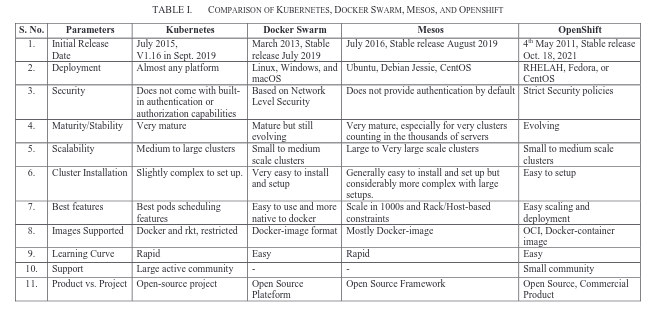
\includegraphics[width=\linewidth]{imagenes/Comparison_Openshift.png}
    \caption{Comparison of Kubernetes, Docker Swarm, Mesos and OpenShift}
    \label{fig:server2}
\end{figure}


\newpage
\subsection*{Análisis Comparativo}
Ahora damos una corporación en forma de tabla donde se detallan las herramientas y la relación con mis objetivos para este proyecto.

\begin{center}
    \begin{tabularx}{\linewidth}{|l|X|X|X|X|} % Ajusta el 'X' para las columnas que necesitan auto-ajuste
        \hline
        \textbf{Características} & \textbf{Docker Swarm} & \textbf{Kubernetes} & \textbf{OpenShift} & \textbf{Apache Mesos} \\
        \hline
        Compatibilidad con HPC & Limitada & Alta, ampliamente adoptado & Alta, diseñado para entornos empresariales & Alta, especialmente en Big Data \\
        \hline
        Despliegue de LLMs & Posible, requiere configuración extra & Ideal para despliegue de aplicaciones complejas, incluyendo LLMs. & Adecuado para LLMs, seguridad reforzada & Escalable, pero no especializado en LLMs \\
        \hline
        Herramientas de SRE & Limitadas & Requiere configuración, pero muy potentes & Integradas (logging, autoscaling, RBAC) & Básicas, depende de configuración manual \\
        \hline
        Escalabilidad & Buena, pero menos flexible & Excelente, diseñado para escalabilidad horizontal y vertical. & Excelente, con alta disponibilidad & Excelente, enfocado en escalabilidad masiva \\
        \hline
        Integración con CI/CD & Requiere herramientas externas & Amplia integración con Jenkins, GitLab... & CI/CD nativo y pipelines predefinidos & Limitada \\
        \hline
        Facilidad de uso & Alta, interfaz simple & Complejo pero flexible y potente & Equilibrado, interfaz gráfica útil & Complejo, curva de aprendizaje elevada \\
        \hline
    \end{tabularx}
\end{center}

\newpage
\begin{multicols*}{2}

\subsection*{Conclusión}
Cada una de las herramientas analizadas tiene sus puntos fuertes y débiles frente a los criterios definidos: desarrollo activo, rendimiento HPC, flexibilidad, herramientas SRE y facilidad de integración CI/CD.

Kubernetes destaca por su flexibilidad y una comunidad activa muy grande. Docker Swarm es fácil de usar y está bien integrado en el ecosistema Docker, pero está más enfocado en aplicaciones de menor escala. Apache Mesos es excelente para manejar grandes clústeres, pero su comunidad reducida y la falta de integración con herramientas sobre SRE lo hacen menos atractivo para este proyecto. Finalmente, OpenShift, basado en Kubernetes, combina seguridad, facilidad de despliegue y automatización, y es una solución de nivel empresarial ideal para entornos HPC.

OpenShift incorpora herramientas de SRE que permiten el monitoreo, el registro de eventos y el escalado automático, facilitando una gestión proactiva de los recursos y la detección temprana de fallos. Estos aspectos son clave para garantizar la disponibilidad y el rendimiento tanto del servidor HPC como de los modelos LLM. Diseñado para entornos empresariales exigentes, permite gestionar aplicaciones complejas con alta eficiencia y continuidad operativa mediante mecanismos de recuperación y escalado dinámico.

Además, su compatibilidad nativa con pipelines de CI/CD agiliza la entrega continua de software, lo que resulta fundamental en proyectos con despliegues frecuentes. Sus funciones de seguridad integradas, como el control de acceso basado en roles y políticas de aislamiento de contenedores, lo hacen especialmente adecuado para entornos sensibles. Por último, aunque Kubernetes ofrece mayor flexibilidad, OpenShift destaca por su interfaz gráfica y sus herramientas integradas de administración, que simplifican considerablemente el despliegue y mantenimiento de clústeres, reduciendo la complejidad operativa.

Finalmente, tengo que mencionar una motivación personal, la universidad me ha ofrecido un curso específico de formación en OpenShift, lo que facilita el proceso de implementación dentro del proyecto. Esta oportunidad permite consolidar los conocimientos técnicos necesarios para aprovechar al máximo esta plataforma, asegurando así una integración más eficiente y alineada con los objetivos del trabajo.

    \section{Análisis Comparativo de Motores de Inferencia para LLM}
    Al trabajar con LLM, necesitamos sistemas que lo hagan funcionar de manera rápida y eficiente, especialmente para aprovechar al máximo la infraestructura en la que están desplegados. En este contexto, los motores de inferencia desempeñan un papel clave, actuando como los “cerebros logísticos” que gestionan estos modelos. Su función principal es organizar y optimizar los recursos disponibles de la forma más eficiente, asegurando así un rendimiento óptimo y un uso inteligente de la infraestructura.
    
    En el presente análisis se exploran tres opciones destacadas: vLLM, TensorRT-LLM de NVIDIA y Text Generation Inference (TGI) de Hugging Face.
    
    \subsection*{vLLM}
    vLLM es un framework de alto rendimiento y código abierto. Fue desarrollado originalmente en la Universidad de California en Berkeley, en colaboración con Neural Magic, empresa que lideraba su mantenimiento y dessarrollo. Desde diciembre de 2024, Red Hat adquirió Neural Magic, convirtiéndose en el principal impulsor comercial del proyecto. A pesar de este cambio, vLLM sigue siendo un proyecto open source, con desarrollo activo en colaboración con la comunidad y la universidad donde se originó
    
    Su principal innovación es el algoritmo PagedAttention, inspirado en las técnicas de paginación de memoria virtual que usan los sistemas operativos. En lugar de asignar grandes bloques contiguos de memoria para la caché clave-valor (KV) ,una estructura esencial en los LLMs, vLLM organiza la memoria en bloques físicos no contiguos y lógicos. Esto reduce significativamente la fragmentación interna y externa de la memoria, un problema común que limita la cantidad de solicitudes que se pueden procesar al mismo tiempo.
    
    Gracias a esta estrategia, vLLM logra un uso casi perfecto de la memoria de la caché KV, con prácticamente cero desperdicio. Además, permite compartir de manera flexible esta caché entre diferentes solicitudes o incluso dentro de una misma solicitud, como ocurre en tareas de generación paralela o búsqueda por haz (beam search). Esta capacidad de compartir memoria de forma inteligente disminuye aún más el consumo total, lo que posibilita manejar más solicitudes en paralelo y mejora el rendimiento general del sistema.
    
    Las evaluaciones presentadas en el artículo Efficient Memory Management for Large Language Model Serving with PagedAttention muestran que vLLM puede aumentar el rendimiento de modelos como OPT y LLaMA entre 2 y 4 veces en comparación con sistemas avanzados como FasterTransformer y Orca, manteniendo niveles de latencia similares. Estas mejoras son especialmente notables en escenarios desafiantes, como secuencias de texto largas, modelos de mayor tamaño y algoritmos de decodificación complejos.
    
    \subsection*{TensorRT-LLM - NVIDIA}
    Pasemos ahora a TensorRT-LLM, desarrollado por NVIDIA y optimizado específicamente para sus GPUs, como las A100 o H100. Este motor está diseñado para ofrecer el máximo rendimiento en hardware NVIDIA, utilizando técnicas avanzadas como la fusión de capas, la cuantización y la ejecución optimizada de kernels CUDA. Estas optimizaciones permiten alcanzar velocidades de inferencia significativamente superiores a las de otros motores más generales.
    
    Por ejemplo, en benchmarks oficiales, TensorRT-LLM logró un rendimiento de aproximadamente 3,679 tokens por segundo con el modelo GPT-J de 6 mil millones de parámetros sobre una GPU A100 de 80 GB . En comparación, vLLM alcanza aproximadamente 714 tokens por segundo con modelos equivalentes como LLaMA-7B en una A100 de 40 GB. Esta diferencia se debe principalmente a las optimizaciones de bajo nivel específicas para GPUs NVIDIA que implementa TensorRT-LLM.
    
    Sin embargo, esta especialización tiene un costo: TensorRT-LLM está limitada a GPUs NVIDIA y requiere que los modelos 

    se conviertan a un formato especial llamado TensorRT Engine, lo que puede añadir complejidad al proceso. Aunque es una herramienta poderosa para quienes ya trabajan con hardware NVIDIA, su falta de flexibilidad la hace menos versátil en comparación con vLLM.
    
    \subsection*{Text Generation Inference (TGI) - Hugging Face}
    Por otro lado, TGI, creado por Hugging Face, se destaca por su capacidad para manejar textos extremadamente largos de manera eficiente.Utiliza técnicas que le permiten recordar información previa sin necesidad de recalcular todo desde cero, lo que ahorra memoria y acelera las respuestas. En pruebas con prompts de más de 200,000 tokens, TGI generó respuestas en solo 2 segundos, mientras que vLLM tardó 27.5 segundos. Además, en una GPU NVIDIA L4, TGI puede manejar hasta 30k tokens, tres veces más que vLLM en configuraciones similares.

    TGI también es muy fácil de usar: con solo especificar el nombre de un modelo de Hugging Face, está lista para funcionar, sin configuraciones complicadas. Aunque está optimizada principalmente para GPUs NVIDIA, su buen desempeño en hardware con recursos limitados la hace atractiva para usuarios con equipos más modestos.

\end{multicols*}

\newpage

\subsection*{Análisis Comparativo}
\begin{center}
\begin{tabularx}{\linewidth}{|l|X|X|X|}
    \hline
    \textbf{Característica} & \textbf{vLLM} & \textbf{TensorRT-LLM (NVIDIA)} & \textbf{Text Generation Inference (TGI) (Hugging Face)} \\
    \hline
    ¿Open Source? & Si & No, es de Nvidia & Si \\
    \hline
    Hardware Principal & Amplia gama de GPUs (NVIDIA, AMD, etc.) & GPUs NVIDIA (optimizado para) & Principalmente GPUs NVIDIA (ejemplo con L4) \\
    \hline
    Optimización Clave & PagedAttention, ahora con soporte de Red Hat & Optimización a nivel de kernel, fusión de capas, gestión dinámica de memoria & Optimización de memoria para prompts largos, retención de contexto, estructuras de datos eficientes \\
    \hline
    Facilidad de Uso & API de Python sencilla, servidor compatible con OpenAI API & Requiere conversión de modelos a formato TensorRT Engine & Cero configuración para la mayoría de los casos, basado en ID de modelo de Hugging Face \\
    \hline
    Rendimiento (vs. vLLM) & 2-4x más rápido que Orca; generalmente más lento que TensorRT-LLM en NVIDIA & Generalmente más rápido y energéticamente eficiente en GPUs NVIDIA & Hasta 13x más rápido en prompts largos (>200k tokens), triplica la capacidad de tokens \\
    \hline
    Manejo de Prompts Largos & Gestión eficiente de memoria KV ayuda & Optimizado para reducir latencia y huella de memoria & Optimizado significativamente, triplica la capacidad de tokens \\
    \hline
    Flexibilidad Hardware & Alta & Limitada a NVIDIA & Principalmente NVIDIA, buena optimización para hardware limitado \\
    \hline
\end{tabularx}
\end{center}
 
\newpage
\subsection*{Conclusión}
\begin{multicols*}{2}

Tras evaluar vLLM, TensorRT-LLM y TGI, vLLM se destaca como la opción más equilibrada en términos de eficiencia, flexibilidad y facilidad de integración. Su algoritmo PagedAttention optimiza el uso de la memoria GPU, permitiendo gestionar múltiples solicitudes concurrentes sin desperdicio de recursos. Por ejemplo, en pruebas con el modelo OPT-13B, vLLM procesó hasta 2.2 veces más solicitudes simultáneas que Orca (Oracle) y 4.3 veces más que Orca (Max), manteniendo latencias similares.

Además, su compatibilidad con hardware diverso (GPUs NVIDIA, AMD, CPUs, TPUs), su naturaleza open source, y el impulso actual de Red Hat como principal contribuidor tras la adquisición de Neural Magic, refuerzan su sostenibilidad a largo plazo y su capacidad de innovación.

Un aspecto especialmente relevante para este Trabajo de Fin de Grado es que vamos a trabajar sobre Red Hat OpenShift como plataforma de orquestación. En este entorno, vLLM está mejor documentado e integrado que otras opciones. Red Hat ha anunciado soporte directo de vLLM en su ecosistema de IA empresarial (incluido en OpenShift AI), facilitando así tanto el despliegue como el escalado automático, el control de recursos y la integración con pipelines de MLOps.

Aunque TensorRT-LLM ofrece un rendimiento superior en hardware NVIDIA y TGI tiene ventajas notables en escenarios con prompts extremadamente largos, vLLM proporciona un rendimiento estable y adaptable, siendo ampliamente utilizado en entornos reales y cada vez más estandarizado. En consecuencia, es la opción más práctica y escalable para un proyecto que busca eficiencia sin comprometer portabilidad ni simplicidad operativa.    

\section{Análisis Comparativo de Modelos LLM}
Una vez elegida OpenShift como plataforma para la gestión del proyecto, el siguiente paso fue determinar qué modelos de lenguaje (LLM) resultaban más adecuados para su implementación en entornos de computación de alto rendimiento (HPC) mediante vLLM. Para ello, se analizaron modelos reconocidos como ChatGPT, Google Gemini, LLaMA y DeepSeek.
\begin{figure}[H]
    \centering
    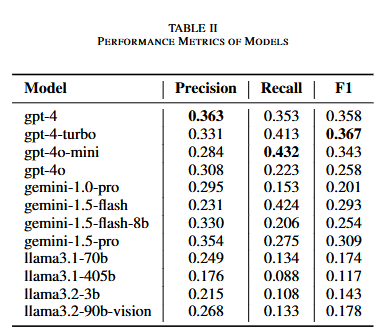
\includegraphics[width=\linewidth]{imagenes/image22.png}
    \caption{}
    \label{fig:server4}
\end{figure}


La evaluación se basó en tres enfoques complementarios. En primer lugar, se revisaron estudios técnicos detallados publicados en artículos científicos, en los cuales se aplicó una metodología zero-shot para tareas de extracción de relaciones en chino, utilizando métricas objetivas como precisión, recall, F1-score y latencia. En segundo lugar, se consideraron resultados normalizados en pruebas estandarizadas ampliamente reconocidas, como MMLU, SAT, LSAT, GRE, TOEFL o GMAT, que permiten medir la capacidad de los modelos en tareas académicas complejas y diversas. Por último, se incorporó la información procedente de Chatbot Arena, una plataforma de evaluación comunitaria basada en comparaciones por pares y votaciones entre modelos, que genera puntuaciones mediante el sistema Elo a partir de más de 2,8 millones de enfrentamientos. Esta combinación de enfoques permite integrar la precisión técnica, el rendimiento en escenarios exigentes y la experiencia práctica de los usuarios en un único análisis comparativo.
\begin{figure}[H]
    \centering
    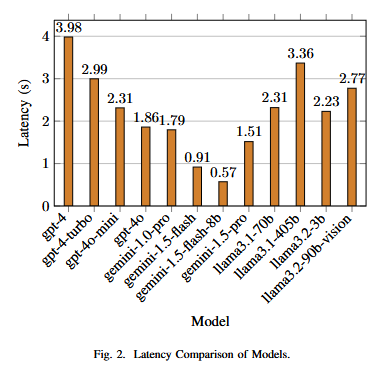
\includegraphics[width=\linewidth]{imagenes/image15.png}
    \caption{}
    \label{fig:server3}
\end{figure}
Chatbot Arena, en particular, resultó ser una herramienta valiosa para evaluar la percepción práctica de los usuarios sobre estos modelos. Con más de 24 millones de votos, la plataforma genera clasificaciones generales mediante un sistema Elo, ofreciendo una visión actualizada y dinámica. Este enfoque destaca diferencias en fluidez, relevancia y coherencia que, en ocasiones, no se evidencian en pruebas más controladas. Por ejemplo, las puntuaciones Elo indican que ChatGPT, especialmente en su versión GPT-4o, alcanza una calificación destacada de aproximadamente 1406, superando a otros modelos y mostrando coherencia con los buenos resultados obtenidos en los análisis técnicos.


\subsection*{ChatGPT}
ChatGPT, desarrollado por OpenAI, alcanzó una gran popularidad tras su lanzamiento en noviembre de 2022. Inicialmente construido sobre GPT-3.5 y posteriormente evolucionado a GPT-4, este modelo emplea una arquitectura de transformador perfeccionada mediante técnicas como el aprendizaje por refuerzo con retroalimentación humana (Reinforcement Learning from Human Feedback, RLHF). Estas mejoras permiten ofrecer respuestas claras, coherentes y adaptadas al contexto, lo que lo ha convertido en una herramienta destacada para la conversación, la redacción de textos y el soporte en programación.

En el estudio de extracción de relaciones en chino, por ejemplo, ChatGPT alcanzó una precisión de aproximadamente 0,363 y un F1-score de 0,358, lo que demuestra su capacidad para generar contenido relevante. No obstante, esta capacidad conlleva un coste: su elevado consumo computacional puede provocar demoras. En el caso de GPT-4, las respuestas pueden tardar hasta 3,98 segundos. En plataformas como Chatbot Arena, los usuarios elogian la calidad de sus respuestas, aunque algunos han señalado que la espera puede representar un inconveniente cuando se requiere inmediatez.

\subsection*{Google Gemini}
Google Gemini, desarrollado por el equipo de DeepMind de Google, fue lanzado en 2023. Este modelo se caracteriza por su arquitectura multimodal, que le permite procesar y generar simultáneamente distintos tipos de datos, incluyendo texto, imágenes y código. En el documento (2502.05694v1.pdf) se muestra que algunas variantes de Gemini, como gemini-1.5-flash-8b, presentan latencias extremadamente bajas, en torno a 0,57 segundos, y precisiones que varían entre 0,295 (gemini-1.0-pro) y 0,354 (gemini-1.5-pro). Esta combinación resulta especialmente atractiva para aplicaciones en tiempo real, donde la velocidad de respuesta es un factor crítico.

Además, las evaluaciones de Chatbot Arena destacan la rapidez de Gemini, situándose en posiciones altas en términos de velocidad. Sin embargo, en comparativas centradas exclusivamente en contenido textual, sus puntuaciones Elo suelen ser algo inferiores a las de ChatGPT, lo que sugiere un compromiso entre velocidad y precisión.

\subsection*{LLaMA}
LLaMA, acrónimo de Large Language Model Meta AI, es un modelo desarrollado por Meta y lanzado en febrero de 2023. Las evaluaciones técnicas en el estudio de extracción de relaciones indican que LLaMA presenta un rendimiento inferior en este contexto. Por ejemplo, la versión llama3.1-405b obtuvo un F1-score de apenas 0,117 y registró una latencia aproximada de 3,36 segundos. Estos resultados evidencian limitaciones significativas tanto en precisión como en eficiencia, lo que se refleja en los rankings generales (overall) de Chatbot Arena, donde la comunidad de usuarios posiciona a LLaMA en un rango inferior en escenarios de alta exigencia.

Esta baja valoración confirma que, tal como se observa en las métricas experimentales, LLaMA requiere ajustes y mejoras sustanciales para competir eficazmente en aplicaciones críticas.

\subsection*{DeepSeek}
DeepSeek, desarrollado por una empresa emergente china, fue introducido a finales de 2023. Se basa en una arquitectura Mixture-of-Experts (MoE) que activa selectivamente los parámetros necesarios para cada consulta, con el objetivo de optimizar la eficiencia computacional. En el documento (2503.04783v1.pdf) se destacan sus capacidades en tareas de razonamiento, codificación y especialización en ámbitos como la salud, el derecho o las finanzas. Por ejemplo, en la tabla de evaluación general de rendimiento, el modelo DeepSeek R1 obtiene una puntuación de 84,0 en MMLU (Overall), frente a 90,0 de ChatGPT GPT-4o y 87,0 de Gemini 1.5 Pro, lo que indica un rendimiento competitivo, aunque ligeramente inferior en tareas generales de razonamiento y conocimiento.

No obstante, DeepSeek alcanza este nivel de rendimiento mediante una arquitectura mucho más eficiente y orientada, lo que lo convierte en una opción especialmente valiosa en entornos con recursos limitados. En la plataforma Chatbot Arena, los usuarios reconocen su excelente rendimiento en dominios específicos, 

\end{multicols*}

\newpage
\noindent
\begin{minipage}[t]{0.48\textwidth} 
    aunque su capacidad de generalización no alcanza los niveles de los modelos más amplios y carece de capacidades multimodales robustas. A pesar de ello, DeepSeek ha logrado posicionarse como el modelo mejor valorado dentro de la categoría de código abierto, lo que representa un logro significativo para una propuesta relativamente reciente en este mercado competitivo.
\end{minipage}%
\hfill 
\begin{minipage}[t]{0.48\textwidth} 
\end{minipage}

\vspace{1em} 
\noindent 


\begin{figure}[H]
    \centering
    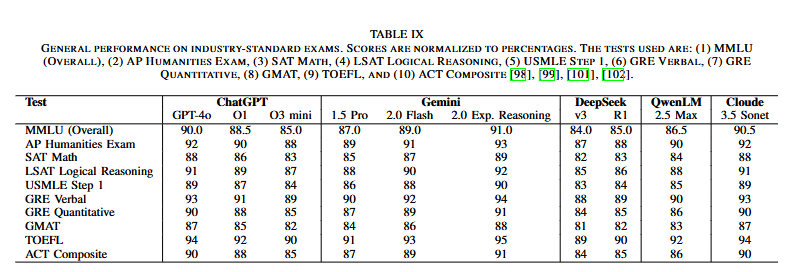
\includegraphics[width=\linewidth]{imagenes/image13.png}
    \caption{}
    \label{fig:server2}
\end{figure}

\newpage

\noindent
\begin{minipage}[t]{0.48\textwidth}
    \subsection*{Analisis Comparativo}
    Una vez presentadas las principales características de los modelos analizados, resulta importante incorporar la evaluación que realiza Chatbot Arena, una plataforma de comparación directa basada en enfrentamientos aleatorios entre modelos. Además del ranking general (Arena Elo), se incluyen benchmarks específicos como MMLU, visto anteriormente (prueba de precisión multitarea en 57 tareas) y Arena-Hard-Auto, una evaluación automática dirigida a modelos adaptados a instrucciones.

    La tabla más reciente de Chatbot Arena, a día que se escribe esta memoria, muestra que ChatGPT-4o y Gemini-2.5-Pro lideran el ranking con valores Elo muy elevados (1406 y 1437, respectivamente), mientras que modelos como DeepSeek-V3 o DeepSeek-R1 presentan rendimientos sólidos pero más discretos (Elo de 1318 y 1359, respectivamente).
\end{minipage}%
\hfill
\begin{minipage}[t]{0.48\textwidth}
    A pesar de ello, DeepSeek-R1 alcanza una puntuación sobresaliente de 90,8 en MMLU, superando a versiones de Gemini 2.0 y situándose cerca del nivel de GPT-4.5 (92,7) o GPT-4o. LLaMA no aparece en los primeros puestos del ranking, aparece con una puntuacion de 1296, siendo el modelo de Llama-3.3-Nemotron-Super-49B-v1, familia de modelo de nvidia pero basado en Llama, se posiciona como el 5 entre modelos open source.

    Esta evaluación empírica confirma que ChatGPT mantiene una posición destacada, no solo por su precisión en entornos controlados, sino también por la preferencia general de los usuarios. Gemini, por su parte, es reconocido por su velocidad y eficiencia multimodal, mientras que DeepSeek se consolida como una opción muy competitiva en precisión multitarea, a pesar de contar con menor visibilidad en el ranking general. En conjunto, la plataforma Chatbot Arena ofrece una perspectiva valiosa al reflejar el rendimiento real y percibido por la comunidad, complementando eficazmente las métricas estáticas tradicionales.
\end{minipage}

\vspace*{0.5em} % Reducido a 0.5em para minimizar el espacio, puedes probar con 0em o un valor negativo si es necesario
\noindent

\begin{figure}[H]
    \centering
    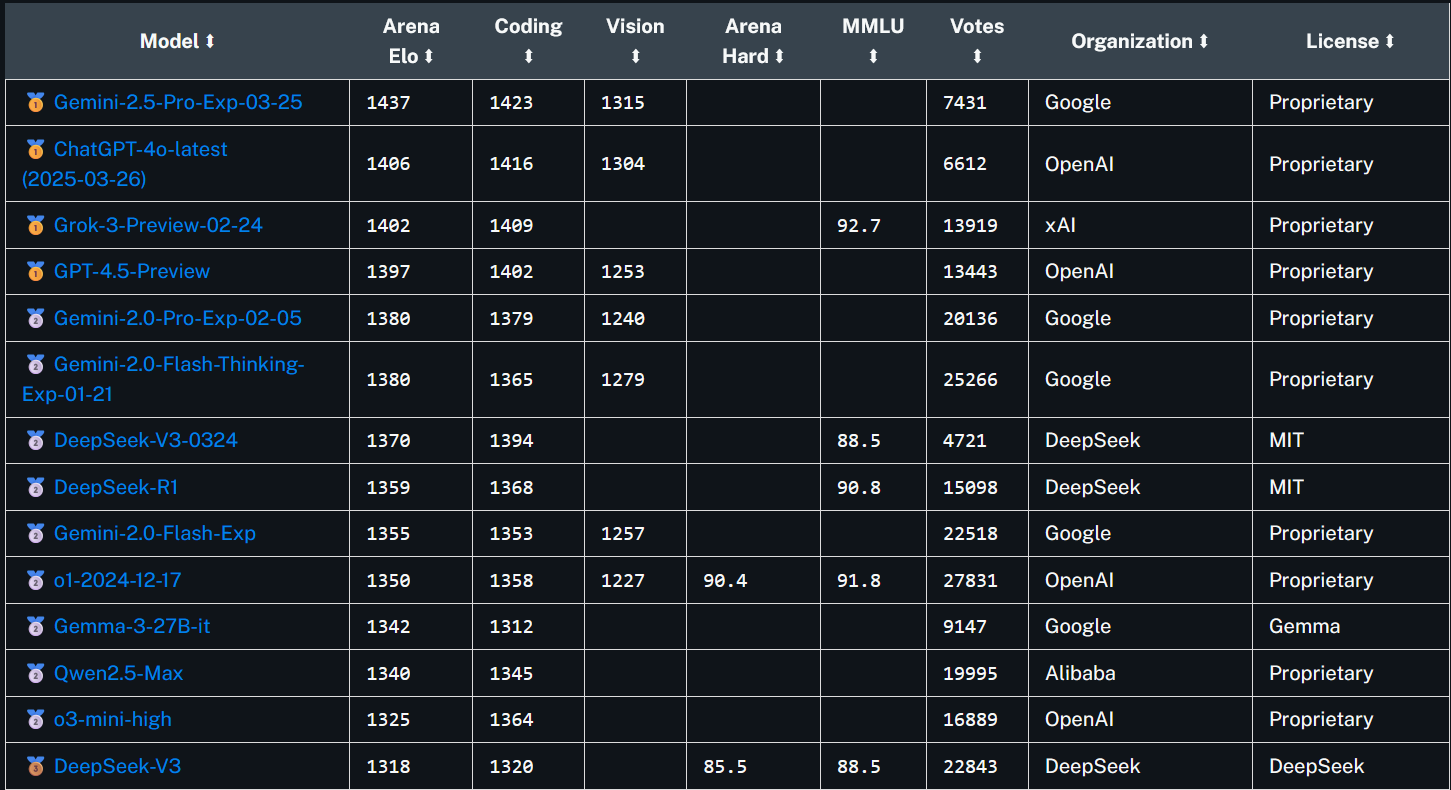
\includegraphics[width=\linewidth]{imagenes/image14.png}
    \caption{}
    \label{fig:server2}
\end{figure}

\newpage
\begin{multicols*}{2}
    \subsection*{Conclusión}
    El análisis realizado permite comprender las fortalezas y limitaciones de los principales modelos LLM en distintos contextos, combinando métricas técnicas con evaluaciones empíricas como las ofrecidas por Chatbot Arena. No obstante, es importante señalar que el ecosistema de modelos evoluciona con gran rapidez: nuevas versiones se publican de forma constante, y un modelo que hoy lidera los rankings puede ser superado en cuestión de semanas.
    
    Aun así, el estudio en profundidad de las características de estos modelos sigue siendo fundamental en el marco de este Trabajo de Fin de Grado, ya que comprender su funcionamiento, eficiencia y adaptación a distintas tareas permite tomar decisiones informadas y anticiparse a futuros desarrollos.
\end{multicols*}

